%\documentclass{article}
%\usepackage{graphicx,subfigure}
%\usepackage{caption,rotating}
%\begin{document}

\begin{figure}[!h]
\centering
\captionsetup{width=0.92\textwidth}
 \subfigure[Sheep 3437 Wrinkled]{
%   \label{fig:trial1he(i)}
%   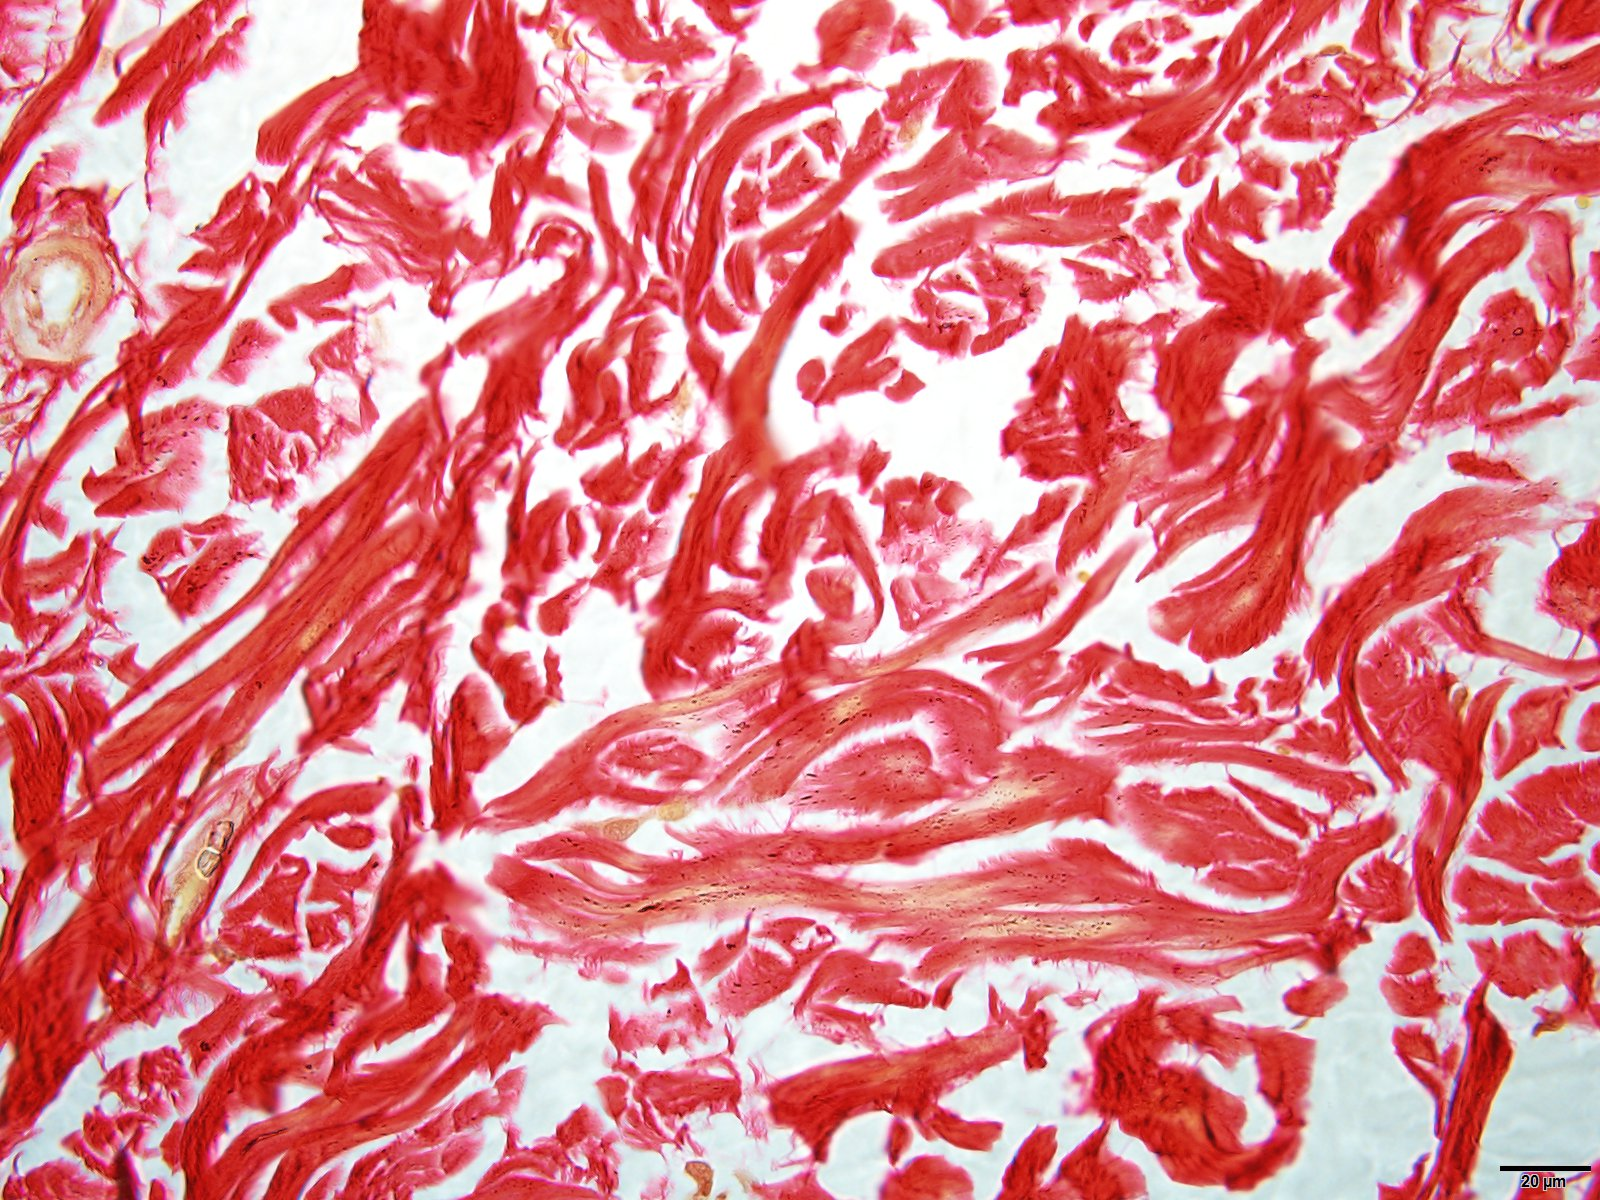
\includegraphics[scale=0.10]{3437_on_wrinkle_1.jpg}
%   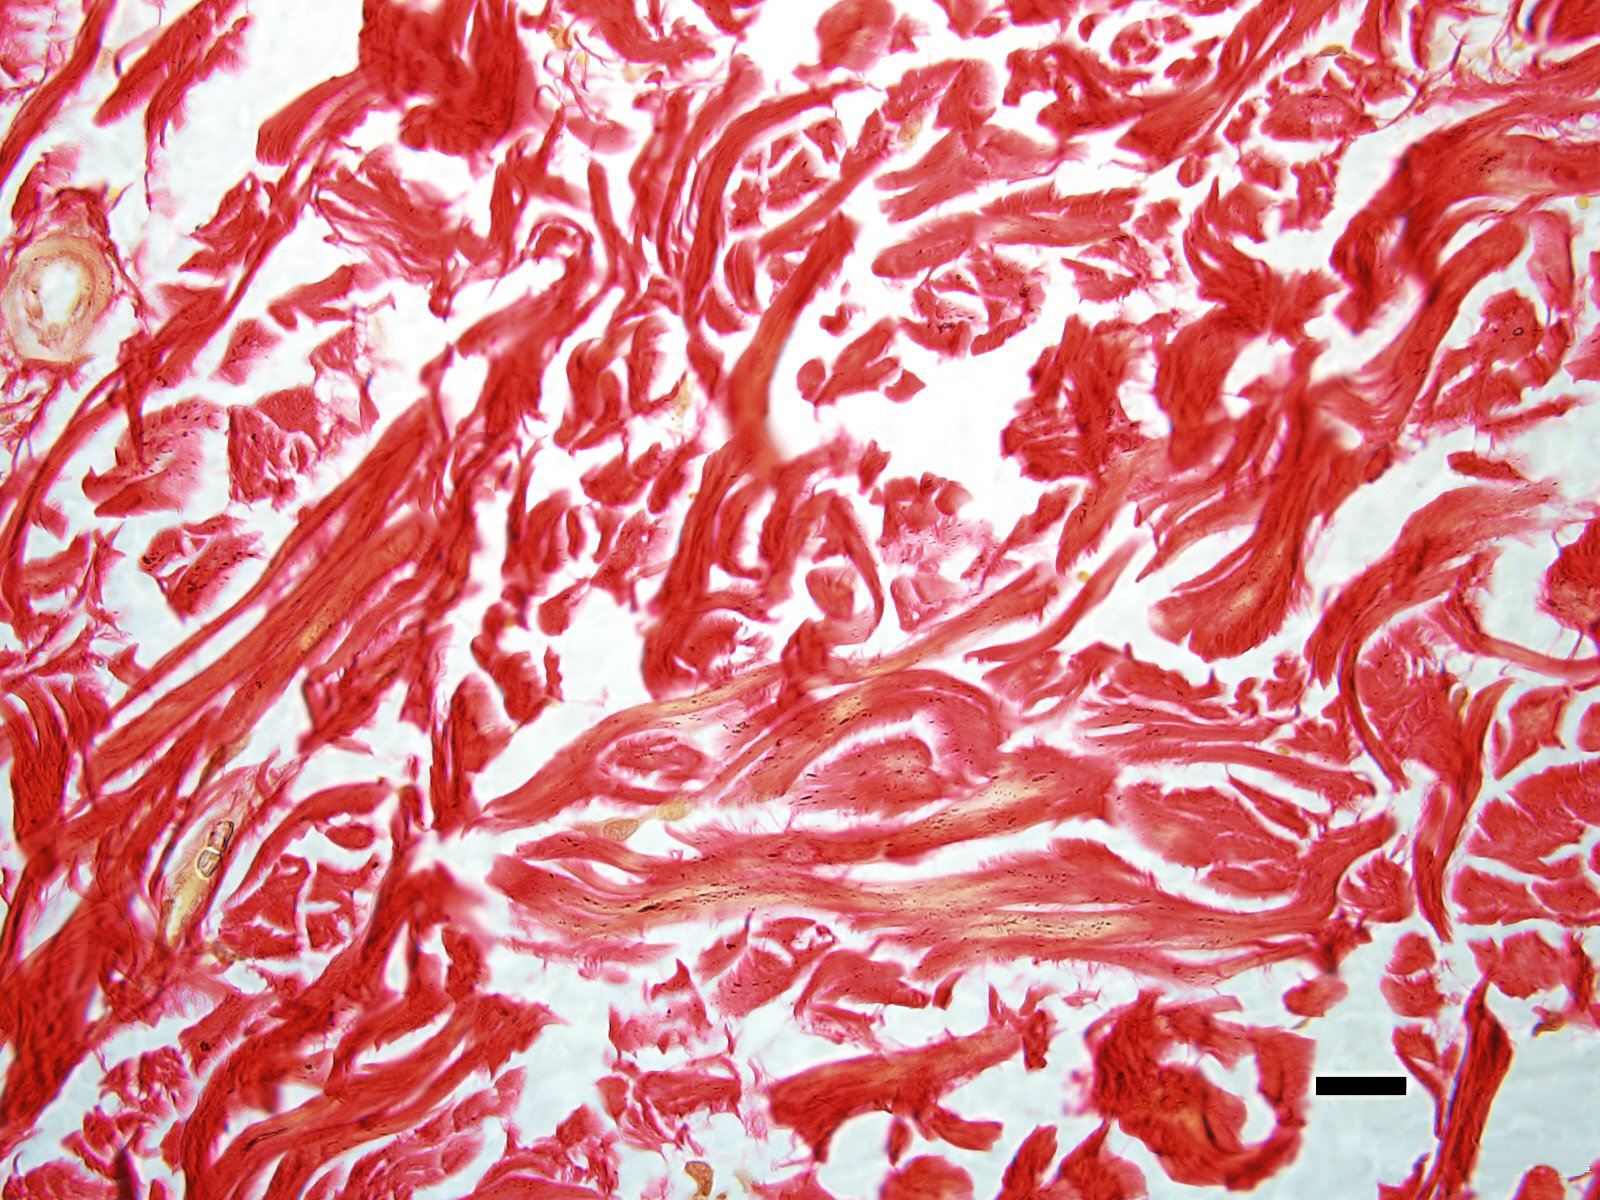
\includegraphics[scale=0.10]{fig5a.jpg}
    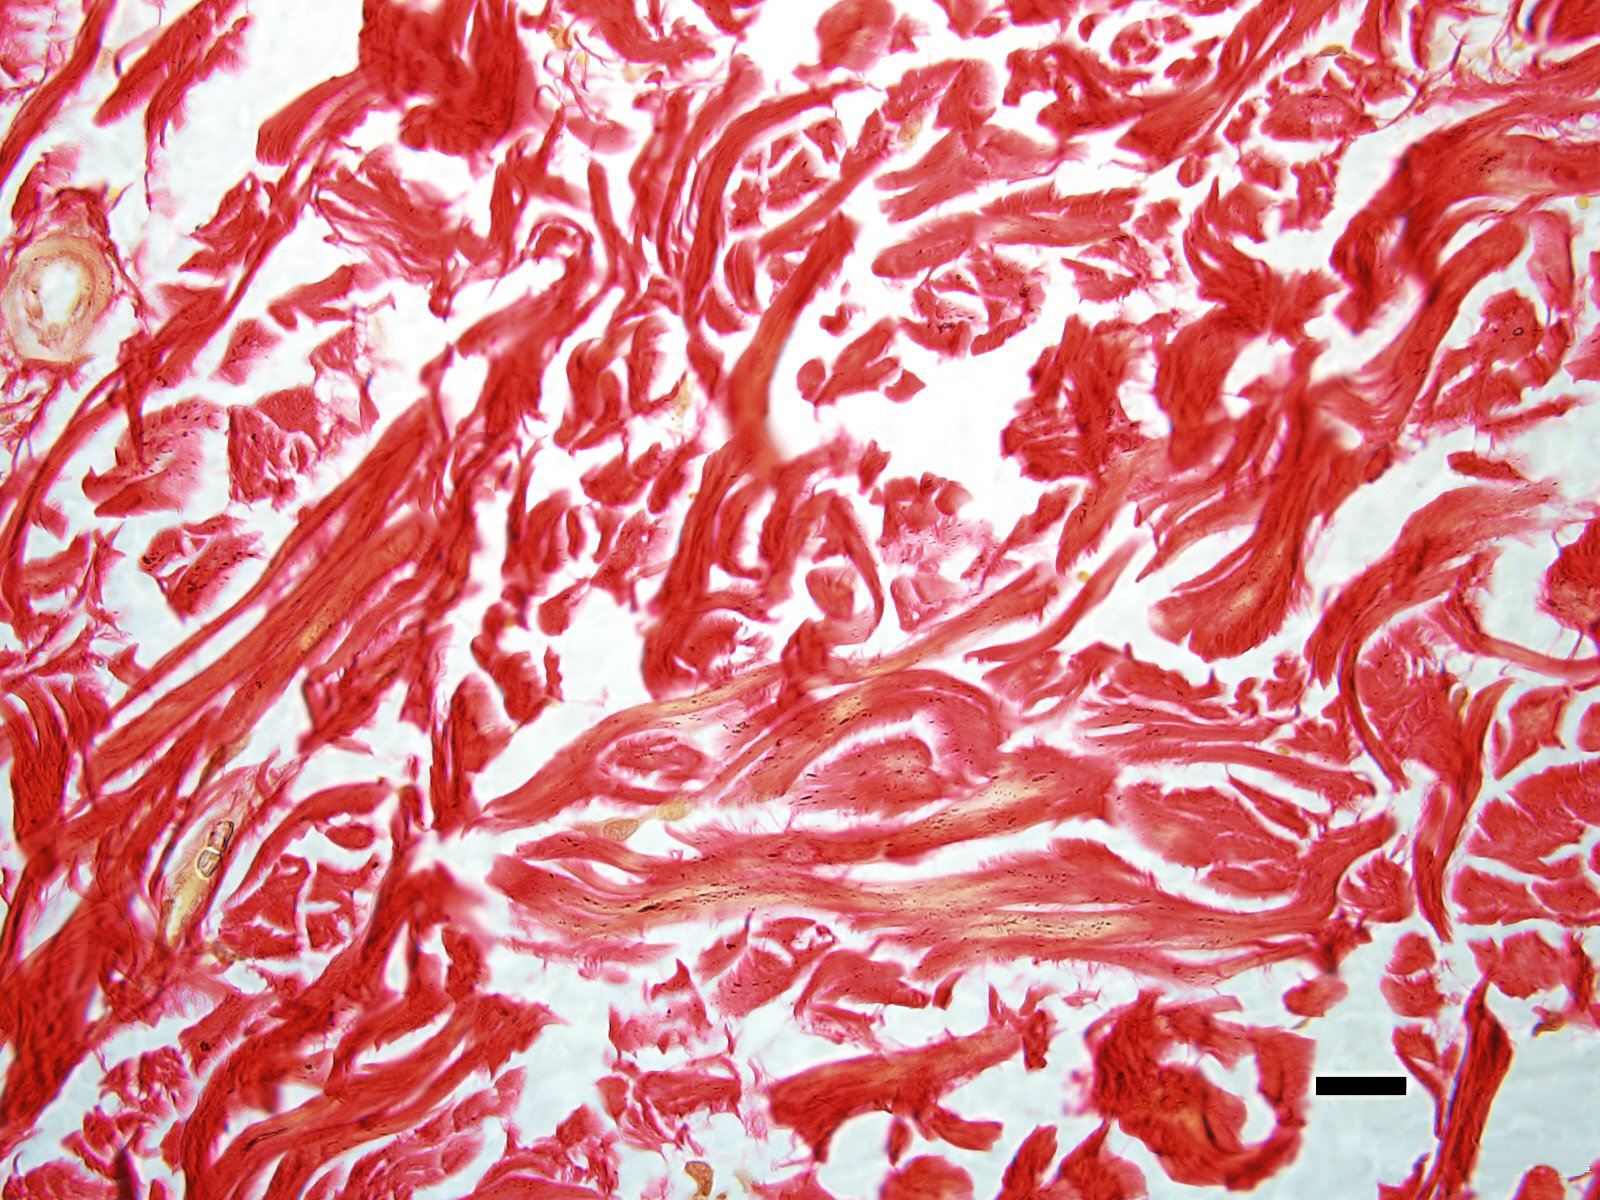
\includegraphics[width=0.46\textwidth]{fig5a.jpg}
% 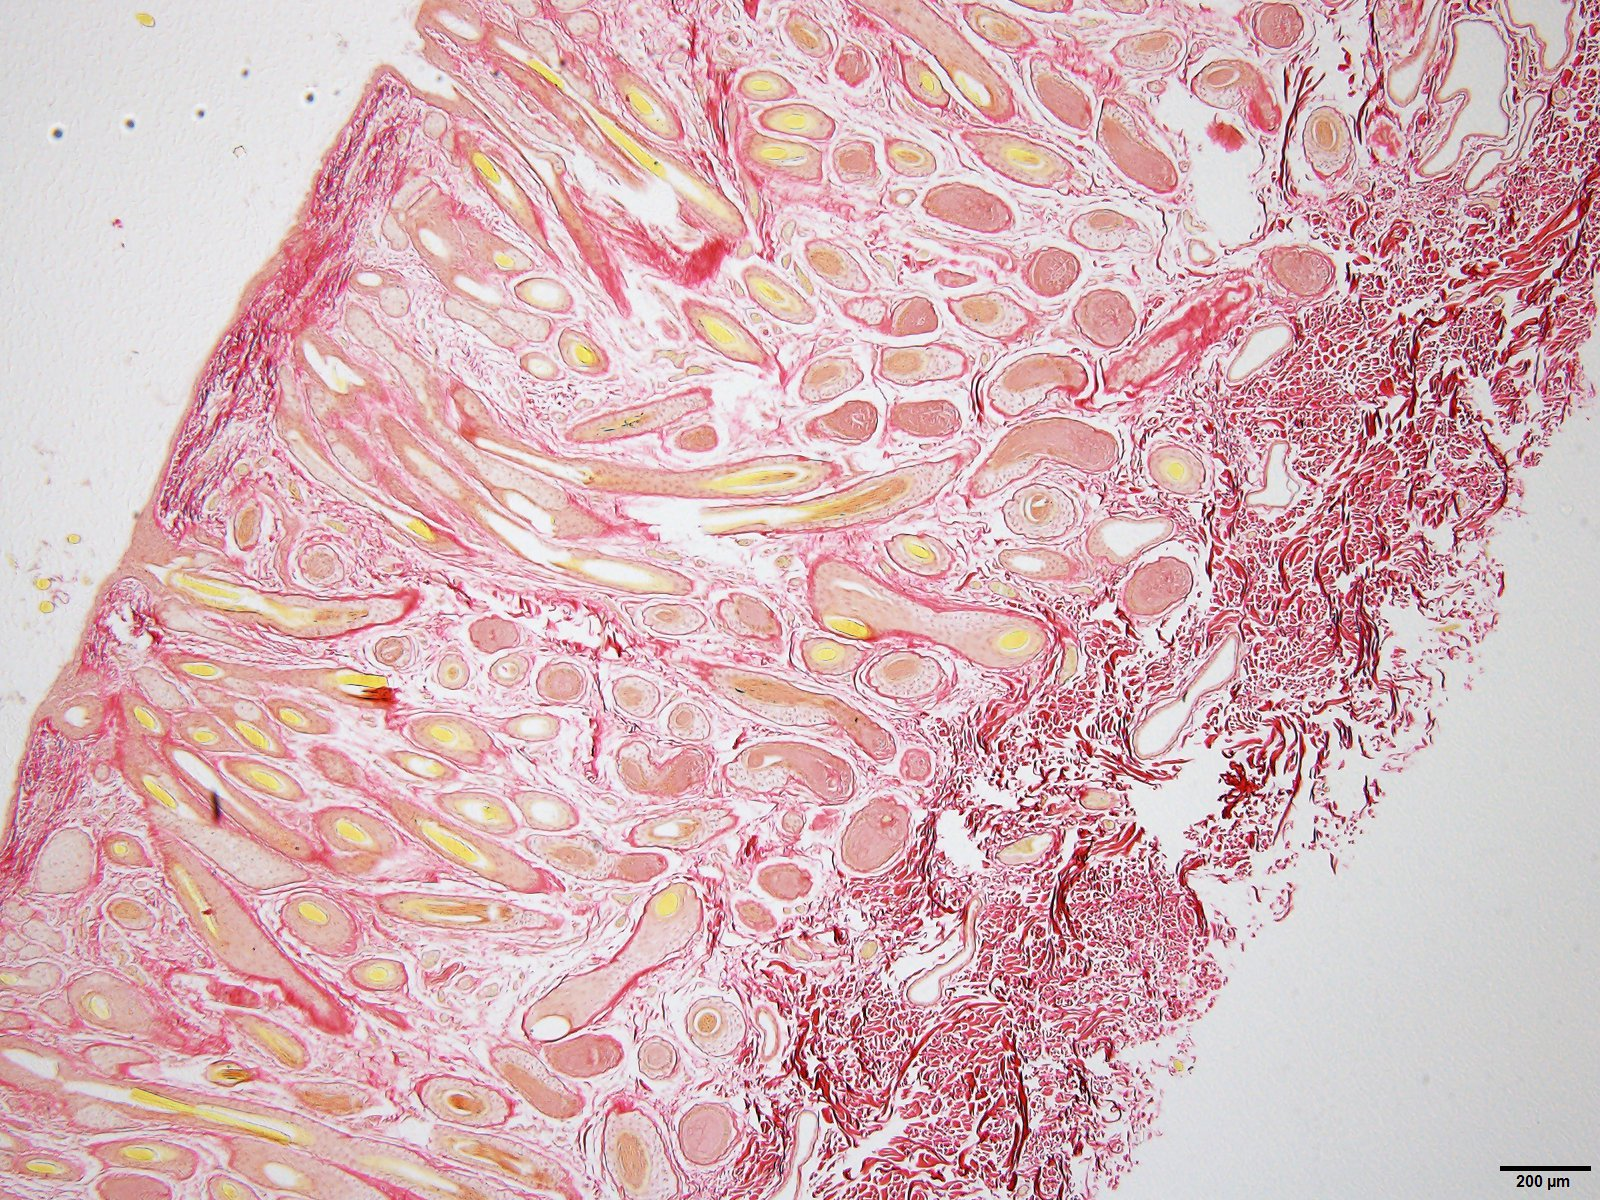
\includegraphics[width=1.0\textwidth]{w479-2-rigid.jpg}
  }
 \subfigure[Sheep 3457 Wrinkle-free]{
%   \label{fig:trial1he(ii)}
%   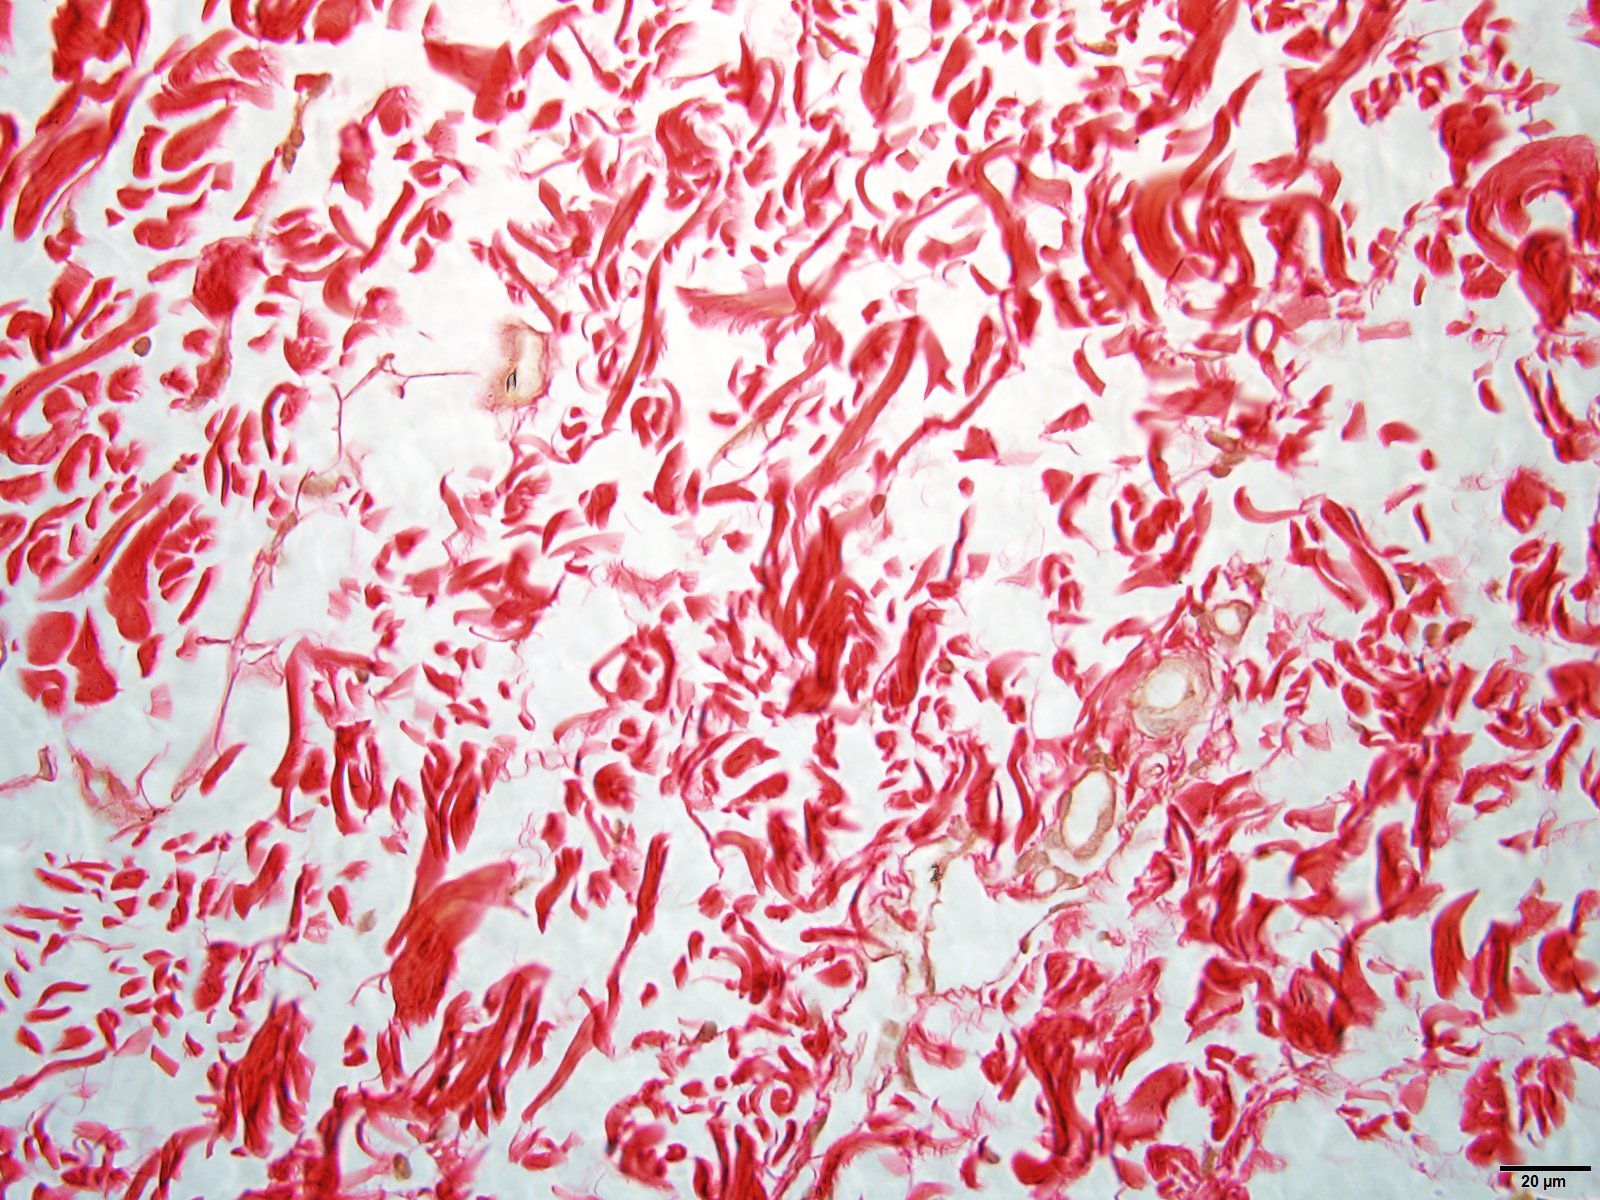
\includegraphics[scale=0.10]{3457_smooth_3.jpg}
%   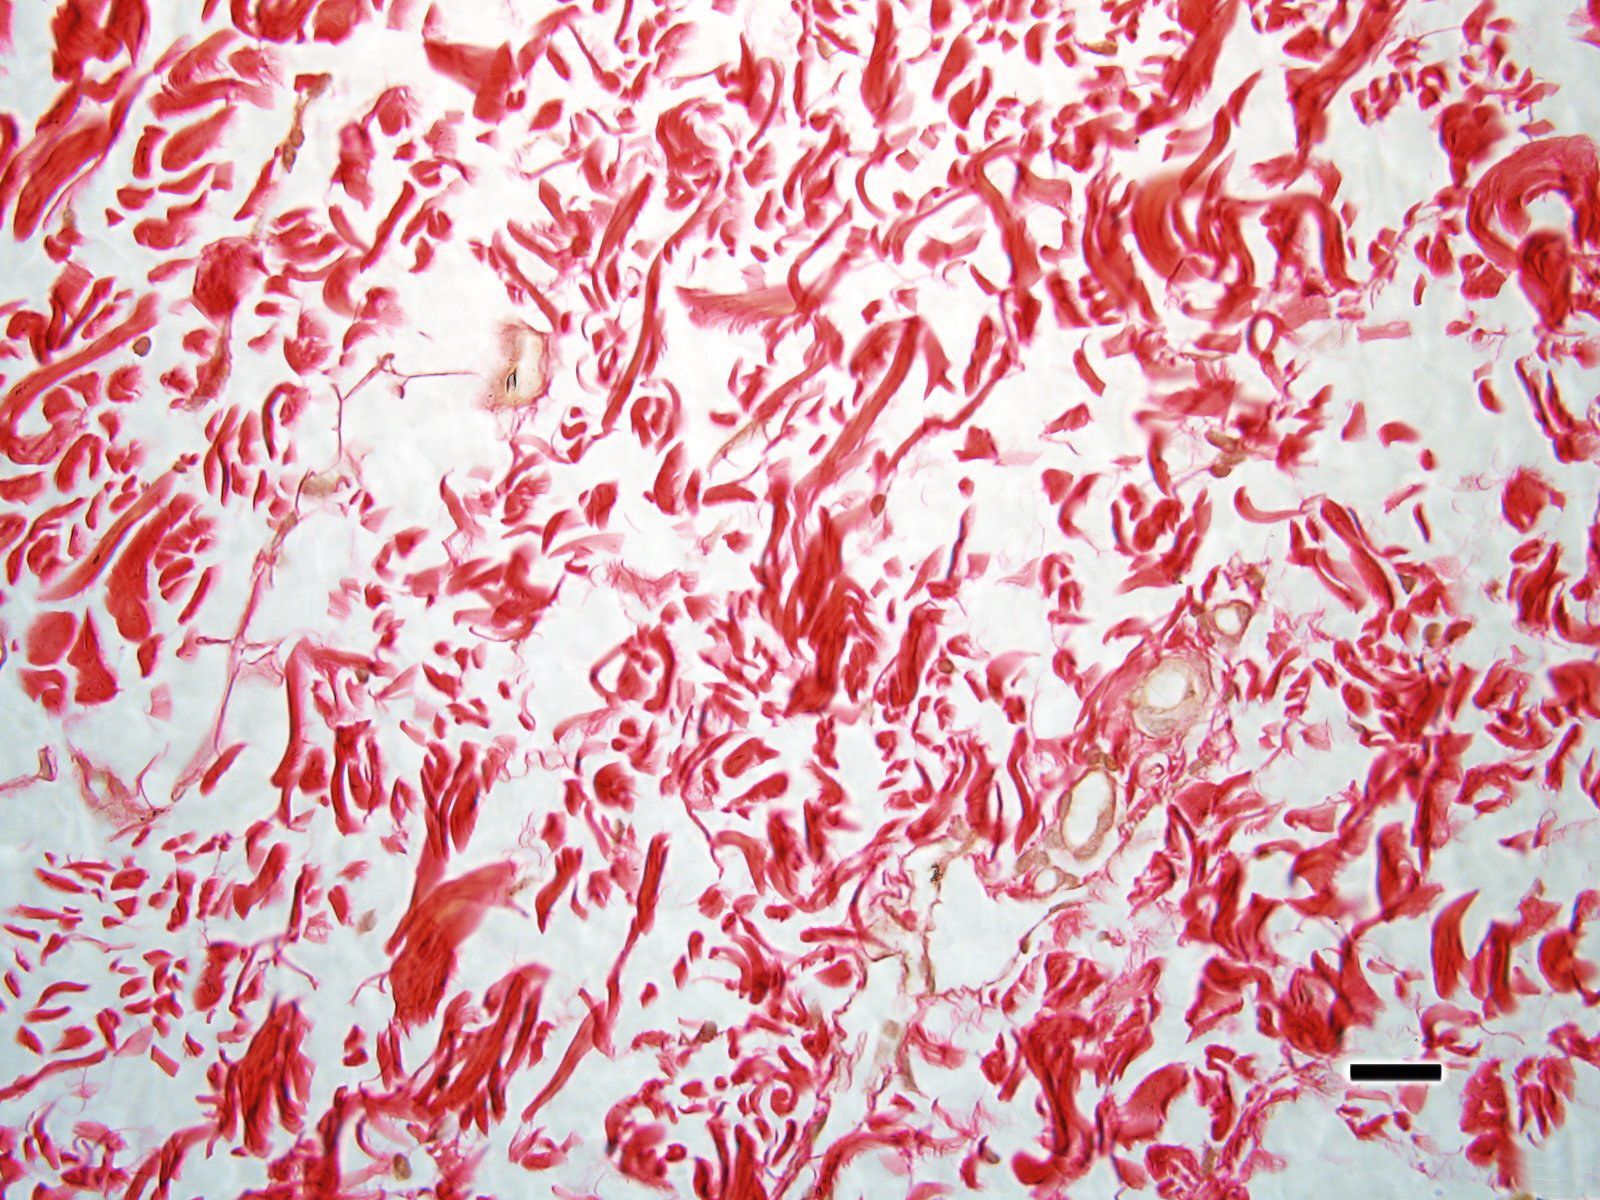
\includegraphics[scale=0.10]{fig5b.jpg}
    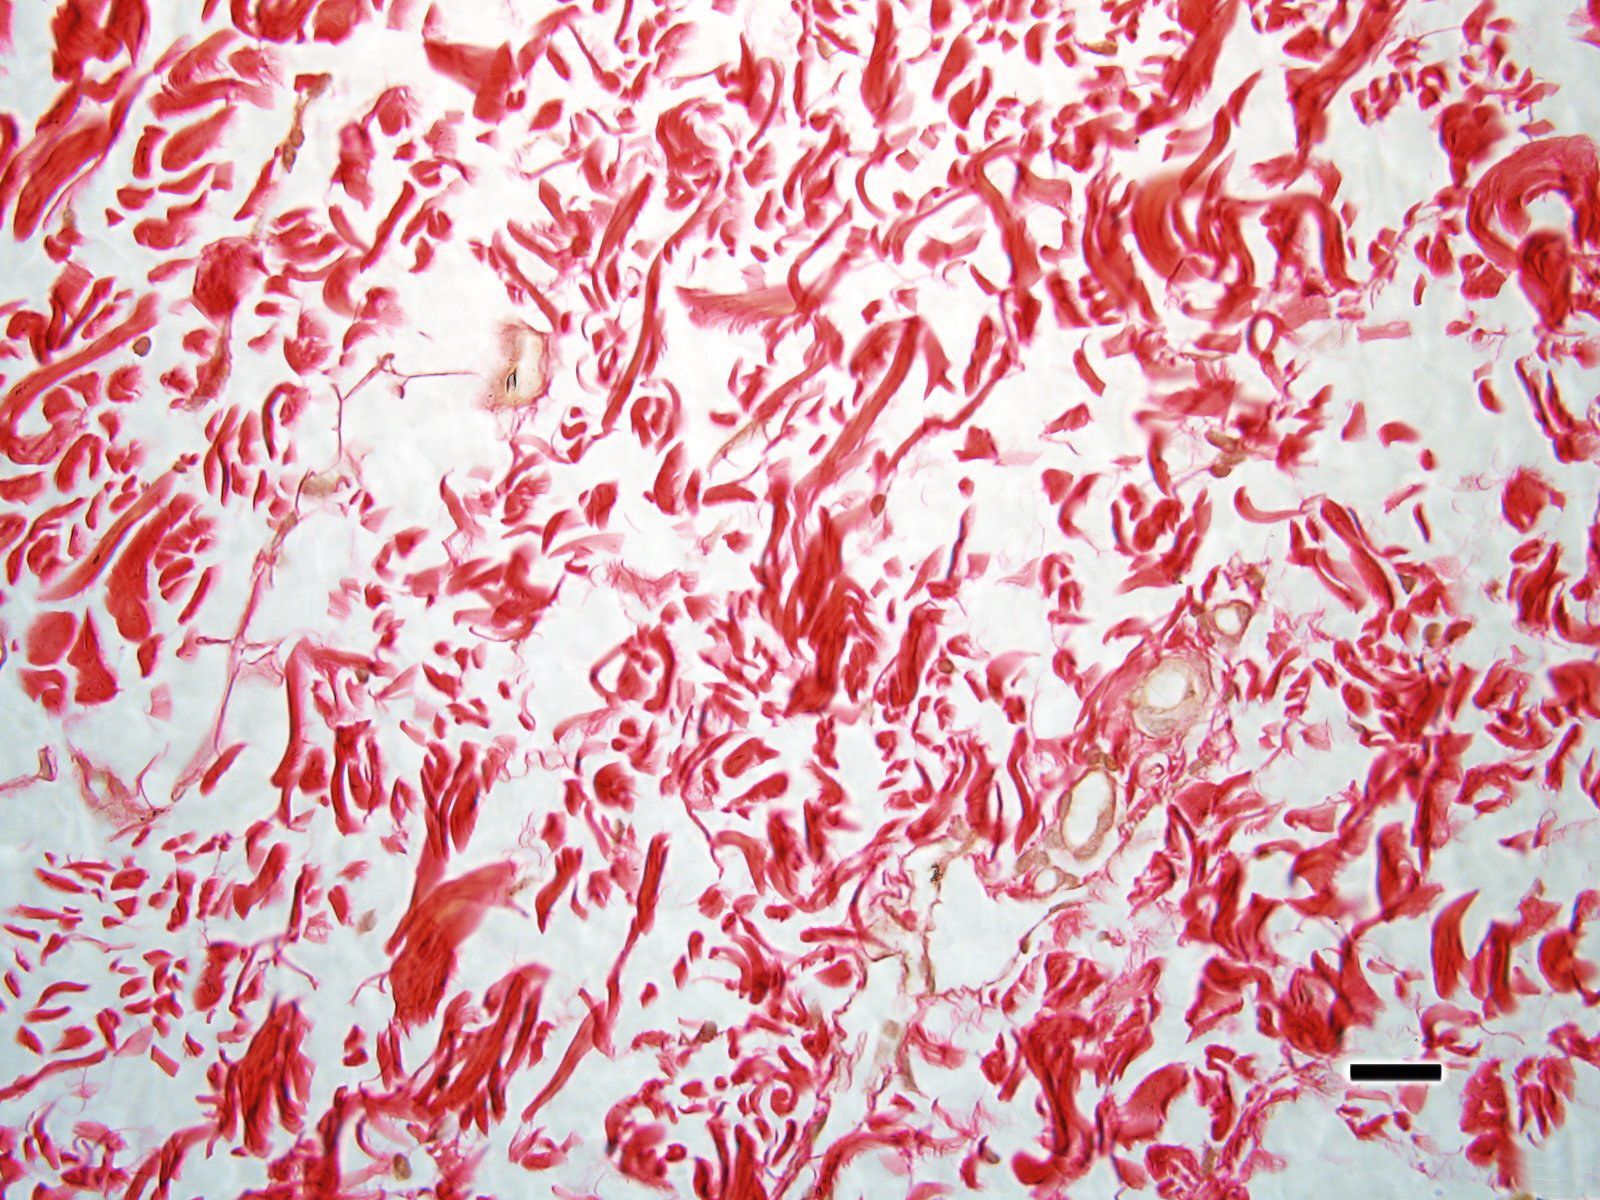
\includegraphics[width=0.46\textwidth]{fig5b.jpg}
  }
  \caption{Fields chosen at random from within Layer 3 (subpapillary dermis) of a wrinkled (a) and a wrinkle-free (b) sheep. Illustrates difference in collagen amount and structure. Stained with PSR and viewed with a 40x objective. Scale bar is $20\mu m$.}
\vfill
  \label{fig:psr40x}
\end{figure}

%\end{document}

